\documentclass[11pt]{article}

\usepackage[utf8]{inputenc}
\usepackage[T1]{fontenc}
\usepackage{lmodern}
\usepackage{microtype}
\usepackage{amsmath,amssymb,booktabs,tabularx,array,multirow}
\usepackage[margin=1in]{geometry}
\usepackage{graphicx}
\usepackage{caption}
\usepackage{subcaption}
\usepackage{enumitem}
\usepackage[numbers,sort&compress]{natbib}
\usepackage[hidelinks]{hyperref}
\usepackage{xurl}
\usepackage{float}
\setlength{\parskip}{0.35em}
\setlength{\parindent}{1em}
\emergencystretch=2em
\captionsetup{font=small,labelfont=bf}
\renewcommand{\abstractname}{Streszczenie}
\renewcommand{\tablename}{Tabela}
\renewcommand{\figurename}{Rysunek}
\renewcommand{\refname}{Literatura}
\newcommand{\comp}{\textsc{comp}}
\newcommand{\coop}{\textsc{coop}}
\newcommand{\equalself}{\texttt{equal\_self}}
\newcommand{\scarce}{\texttt{scarce}}
\newcommand{\abundant}{\texttt{abundant}}
\newcommand{\logit}{\operatorname{logit}}

\title{Wpływ niedoboru zasobów na wybory rywalizacyjne modeli językowych o otwartych wagach}
\author{Jacek Rozwadowski\\[2pt]\normalsize Independent Researcher, EdgeNodeLab}
\date{Listopad 2026}

\begin{document}
\maketitle

\begin{abstract}
Sprawdzamy, czy sposób przedstawienia sytuacji decyzyjnej w tekście promptu zmienia wybory modeli językowych o otwartych wagach, gdy struktura wypłat pozostaje niezmieniona. Zadaniem jest jednorazowy wymuszony wybór A/B między działaniem rywalizacyjnym a kooperacyjnym; mierzymy względny logit kolejnego tokenu, uśredniony po obu kolejnościach opcji. Przebadano 12 wariantów modeli (Base i Instruct z rodzin Qwen2.5 w trzech rozmiarach, Mistral-7B, Bielik-11B-v3 i Gemma-4-12B), dwa języki (angielski i polski), trzy określenia aktora, trzy opisy działań, pięć struktur wypłat i dwa konteksty dostępności zasobów (41\,472 oceny). Wnioskowanie opiera się na szablonach parafraz, a nie na pojedynczych promptach. Siedem wariantów przeszło kontrole poprawności pomiaru (masa prawdopodobieństwa na A/B oraz trafność w kontrolach dominacji); pozostałe pięć wyłączono z analizy głównej, a ich wyniki podajemy w analizie wrażliwości.

W głównym warunku równych wypłat własnych (\equalself) zdanie o niedoborze zasobów zwiększa logit wyboru rywalizacji we wszystkich siedmiu uwzględnionych wariantach (od 0.15 do 1.93 logitu; w skali prawdopodobieństwa od 2.3 do 12.9 punktu procentowego); w sześciu z nich efekt spełnia próg Bonferroniego (0.0018), w Qwen2.5-14B-Instruct jest nominalnie istotny, ale progu nie przekracza. Znak efektu jest dodatni także w pozostałych pięciu, wyłączonych wariantach. W Qwen2.5-3B i 7B efekt jest znacznie większy w wariantach Instruct niż Base, lecz warianty te korzystały z różnych protokołów promptowania, a w Qwen2.5-14B-Instruct efekt jest mały, więc różnicy nie można przypisać dostrajaniu instrukcyjnemu. Kierunek efektu nacechowanego opisu działań (\texttt{charged} vs.\ \texttt{plain}) i efekty określenia aktora nie są spójne między modelami. Eksploracyjna analiza kontroli dominacji wskazuje, że opisy „samodzielnie”/„wspólnie” przesuwają wybory w stronę opcji kooperacyjnej w sześciu z siedmiu wariantów, a neutralne etykiety X/Y -- nie.

Wyniki dotyczą warunkowych rozkładów kolejnego tokenu w sztucznych promptach, a nie celów ani trwałych preferencji modeli. Kryterium kwalifikacji modeli zmieniono po zobaczeniu wcześniejszych wyników, modele dodawano w kolejnych przebiegach, a wnioskowanie opiera się na sześciu parafrazach na język; wnioski traktujemy jako wstępne.
\end{abstract}

\noindent\textbf{Słowa kluczowe:} duże modele językowe; decyzje społeczne; współpraca; rywalizacja; ujęcie sytuacji jako niedoboru;
wrażliwość na prompt; ocena na podstawie logitów; ewaluacja dwujęzyczna

\section{Wprowadzenie}
Duże modele językowe (LLM) są coraz częściej wykorzystywane w procesach, w których ich rekomendacje mogą wpływać na sytuację wielu zainteresowanych stron. Ich zachowanie w warunkach podejmowania decyzji strategicznych i mających konsekwencje społeczne stanowi zatem problem wymagający empirycznego zbadania, a nie czegoś, co można wywnioskować wyłącznie na podstawie płynności generowanego języka. W ostatnich latach badania obejmowały zachowanie modeli LLM w powtarzanych grach, jednorazowych dylematach społecznych oraz zadaniach wymagających koordynacji działań. Wyniki tych prac wskazują zarówno na zdolność modeli do użytecznego dostosowywania strategii, jak i na znaczną wrażliwość ich zachowania na strukturę zadania oraz sposób przedstawienia sytuacji \citep{phelps2025machine,akata2025repeated,tewolde2026coopeval,pal2026robust}.

Jednym z powracających problemów metodologicznych jest trudność w oddzieleniu rzeczywistej preferencji współpracy od innych czynników, takich jak zdolność modelu do poprawnego odczytywania tabel wypłat, nacechowanie semantyczne opisów działań czy skłonność do wybierania pierwszej lub drugiej opcji. Model, który wybiera działanie opisane jako kooperacyjne, może reagować przede wszystkim na użyte sformułowania, a nie na strukturę wypłat. Z drugiej strony model, który nie przechodzi testu dominacji wypłat, może sprawiać wrażenie prosocjalnego jedynie dlatego, że niepoprawnie porównuje wartości liczbowe.

W niniejszym badaniu zastosowano sparowany schemat wymuszonego wyboru, który pozwala rozdzielić wpływ kilku z tych czynników. Główną zmienną wynikową jest względne prawdopodobieństwo przypisywane opcjom rywalizacyjnym i kooperacyjnym, szacowane na podstawie logitów kolejnego tokenu odpowiadającego etykietom odpowiedzi. Każdy scenariusz prezentowany jest dwukrotnie, z odwróconą kolejnością opcji. Zastosowano również dwie kontrolne struktury wypłat oparte na dominacji, które pozwalają sprawdzić, czy model potrafi wybrać opcję korzystną dla obu stron niezależnie od tego, czy jej opis sugeruje rywalizację, czy współpracę. Główny warunek badania, oznaczony jako \equalself, utrzymuje wypłatę decydenta na jednakowym poziomie dla obu możliwych działań, jednocześnie sprawiając, że rywalizacja prowadzi do pogorszenia wyniku drugiej strony.

Badanie koncentruje się na trzech hipotezach i jednym pytaniu eksploracyjnym:

\begin{enumerate}[leftmargin=2.4em,itemsep=0.15em,label=\textbf{H\arabic*:}]
    \item Nacechowany opis działań (\texttt{charged}) zmniejsza w porównaniu z opisem \texttt{plain} prawdopodobieństwo wyboru rywalizacji w warunku \equalself{} (hipoteza wynikła z wcześniejszych obserwacji, por.\ rozdz.~\ref{sec:stats}).
    \item Określenie aktora (plemię, zespół, agent) systematycznie wpływa na wybory rywalizacyjne.
    \item Informacja o niedoborze zasobów zwiększa prawdopodobieństwo wyboru rywalizacji, gdy deklarowane wypłaty pozostają niezmienione (hipoteza również wynikła z wcześniejszych obserwacji).
    \item[\textbf{Q:}] Jak duże są przesunięcia wyborów wynikające ze sposobu sformułowania w porównaniu z wpływem jednoznacznie dominujących wypłat liczbowych? (analiza eksploracyjna)
\end{enumerate}

Najbardziej powtarzalnym wynikiem jest dodatni wpływ przedstawienia sytuacji jako niedoboru zasobów, zaobserwowany we wszystkich siedmiu wariantach modeli, które przeszły przyjęte procedury diagnostyczne (w sześciu z nich po korekcji Bonferroniego). Efekty związane ze sposobem opisu działań i określeniem aktora są natomiast znacznie mniej jednorodne. Podkreślamy, że eksperyment mierzy odpowiedzi modeli uwarunkowane treścią promptu, w sztucznie skonstruowanym scenariuszu jednorazowej decyzji dotyczącej podziału zasobów. Nie stanowi on dowodu na istnienie u modeli wewnętrznych preferencji, intencji ani autonomicznych celów społecznych.

\section{Przegląd dotychczasowych badań}
\paragraph{Sposób formułowania promptów a preferencje społeczne.}
Phelps i Russell badają, czy opisy wyrażające postawy kooperacyjne, rywalizacyjne, altruistyczne i skoncentrowane na własnym interesie mogą zmieniać zachowanie modelu GPT-3.5 w powtarzanym dylemacie więźnia oraz w grze dyktatora. Autorzy wskazują, że opisy postaci oparte na języku naturalnym mogą przekładać się na odpowiadające im zachowania w zadaniach, szczególnie w sytuacjach jednorazowych \citep{phelps2025machine}. Zastosowana w naszym badaniu manipulacja językowa ma węższy zakres: zmienia opisy dwóch dostępnych działań, pozostawiając ich wypłaty bez zmian. Dodatkowo uwzględnia neutralne etykiety działań jako warunek odniesienia.

\paragraph{Modele językowe w grach strategicznych.}
Akata i współautorzy wykorzystują metody behawioralnej teorii gier do oceny modeli językowych w skończenie powtarzanych grach dwuosobowych. Wskazują na różnice między grami opartymi na interesie własnym a zadaniami wymagającymi koordynacji, a także na wrażliwość modeli na dodatkowe informacje społeczne \citep{akata2025repeated}. Pal i współautorzy analizują strategie w powtarzanym dylemacie więźnia, zróżnicowanie wypłat oraz alternatywne sposoby przedstawienia sytuacji. Ich wyniki wskazują, że współczesne modele mogą wykazywać spójne strategie kooperacyjne w określonych warunkach, jednak nie zachowują pełnej konsekwencji we wszystkich badanych wariantach \citep{pal2026robust}. Wspomniane badania dotyczą interakcji powtarzanych i dostosowywania strategii w kolejnych rundach, podczas gdy niniejszy eksperyment koncentruje się na pojedynczym wyborze przy z góry określonych wypłatach dla obu stron.

Tewolde i współautorzy przedstawiają CoopEval – zestaw testów obejmujący kilka rodzajów dylematów społecznych oraz mechanizmy sprzyjające podtrzymywaniu współpracy. W przeprowadzonych eksperymentach zaobserwowali znaczny udział zachowań polegających na rezygnacji ze współpracy w jednorazowych grach o mieszanej motywacji, wśród badanych przez nich modeli. Wykazali również, że mechanizmy instytucjonalne mogą wpływać na wyniki związane ze współpracą \citep{tewolde2026coopeval}. Zadanie zastosowane w naszym badaniu nie jest dylematem więźnia ani powtarzaną grą strategiczną. Polega na jednostronnym wyborze między dwoma możliwymi wynikami, określonymi z perspektywy decydenta oraz drugiej strony. Ta prostsza struktura pozwala na bezpośrednie manipulowanie wypłatą decydenta, wypłatą drugiej strony oraz kontekstem i sposobem sformułowania opisu sytuacji.

\paragraph{Miejsce i wkład niniejszego badania..}
Celem pracy jest wniesienie wkładu przede wszystkim metodologicznego i diagnostycznego, a nie stworzenie ogólnego rankingu modeli językowych pod względem ich skłonności do zachowań prospołecznych. Zastosowany schemat badawczy łączy pięć elementów: 
(i) odwracanie kolejności prezentowanych opcji, (ii) kontrolne scenariusze z dominującymi strukturami wypłat, (iii) warunek równych wypłat własnych decydenta, (iv) neutralne i nacechowane semantycznie opisy działań oraz (v) szablony parafraz w języku angielskim i polskim. Uzyskane wyniki pozwalają ocenić, czy wpływ sposobu przedstawienia sytuacji utrzymuje się również wtedy, gdy model wykazuje zdolność do poprawnego rozpoznawania liczbowej relacji dominacji w warunku wykorzystującym neutralne etykiety działań.

\section{Projekt eksperymentu}
\subsection{Zadanie i struktury wypłat}
Każdy prompt opisuje sytuację, w której dwie strony korzystają ze wspólnej puli zasobów. Decydent musi wybrać między działaniem rywalizacyjnym a działaniem kooperacyjnym. Wynik każdego działania przedstawiany jest jako uporządkowana para wartości \((u_{\mathrm{self}},u_{\mathrm{other}})\), gdzie pierwsza wartość oznacza wypłatę strony podejmującej decyzję, a druga – wypłatę drugiej strony.

Zadanie ma postać jednorazowego scenariusza decyzyjnego, w którym jedna strona dokonuje wyboru na podstawie określonych wypłat. Nie modeluje ono jednoczesnego podejmowania strategicznych decyzji przez dwóch graczy.

W eksperymencie zastosowano pięć struktur wypłat. Trzy z nich stanowią właściwe warunki badawcze, a dwie pełnią funkcję kontroli dominacji. Właściwe warunki badawcze oceniano przy zastosowaniu dwóch skal wypłat (mnożniki 1 i 2), natomiast w przypadku warunków kontrolnych zastosowano tylko jedną skalę.

\begin{table}[H]
\centering
\small
\caption{Struktury wypłat. Każda uporządkowana para oznacza (wypłatę decydenta, wypłatę drugiej strony).}
\begin{tabular}{lccp{5.6cm}}
\toprule
Warunek & Działanie rywalizacyjne & Działanie kooperacyjne & Interpretacja \\
\midrule
\texttt{comp\_dominant} & $(8,3)$ & $(5,5)$ & Rywalizacja zwiększa wypłatę decydenta, jednocześnie zmniejszając wypłatę drugiej strony. \\
\texttt{coop\_dominant} & $(5,3)$ & $(8,8)$ & Współpraca przynosi korzyści obu stronom w porównaniu z rywalizacją. \\
\texttt{equal\_self} & $(6,2)$ & $(6,6)$ & Wypłata decydenta jest identyczna dla obu działań; rywalizacja zmniejsza wypłatę drugiej strony. \\
\texttt{dom\_comp} & $(8,8)$ & $(4,3)$ & Działanie rywalizacyjne jest ściśle korzystniejsze dla obu stron (kontrola dominacji). \\
\texttt{dom\_coop} & $(4,3)$ & $(8,8)$ & Działanie kooperacyjne jest ściśle korzystniejsze dla obu stron (kontrola dominacji). \\
\bottomrule
\end{tabular}
\label{tab:payoffs}
\end{table}


Warunek \equalself{} stanowi główny warunek analizy wyników. Ponieważ oba działania zapewniają decydentowi wypłatę w wysokości 6 jednostek, preferencji dla działania rywalizacyjnego nie można wyjaśnić wyższą deklarowaną wypłatą własną. Taki wybór może jednak wynikać ze sposobu interpretacji promptu, skojarzeń semantycznych, obciążenia odpowiedzi określoną preferencją lub innych, nieobserwowanych mechanizmów działania modelu. Konstrukcja zadania nie pozwala ustalić, która z tych przyczyn odpowiada za dokonany wybór.

\subsection{Czynniki eksperymentalne}
Generator promptów łączy następujące czynniki eksperymentalne:

\begin{itemize}[leftmargin=1.5em,itemsep=0.1em]
\item \textbf{Język:} angielski i polski.
\item \textbf{Sposób określenia uczestników:} agenci (Agent A i Agent B), zespoły (zespół decydenta i drugi zespół) lub plemiona (plemię decydenta i plemię rywali).
\item \textbf{Sposób opisu działań:} \texttt{charged}, \texttt{plain} lub \texttt{label}.
\item \textbf{Struktura wypłat:} pięć warunków przedstawionych w tabeli~\ref{tab:payoffs}.
\item \textbf{Kontekst sytuacyjny:} zdanie wskazujące na niedobór zasobów (zasobów nie wystarczy dla wszystkich) lub ich obfitość (zasobów jest więcej, niż potrzeba dla wszystkich).
\item \textbf{Szablon:} sześć parafraz dla każdego języka.
\item \textbf{Kolejność opcji:} najpierw opcja rywalizacyjna lub najpierw opcja kooperacyjna.
\end{itemize}

Trzy warianty opisu działań celowo różnią się zawartością semantyczną. W promptach angielskich wariant \texttt{charged} zestawia sformułowania „Seize control of the pool and push the other side out” (pol.\ przejąć kontrolę nad pulą i wypchnąć drugą stronę) oraz „Join forces with the other side and manage the pool together” (pol.\ połączyć siły z drugą stroną i zarządzać pulą wspólnie). Wariant \texttt{plain} zestawia „Act on the pool independently” (pol.\ działać na puli samodzielnie) oraz „Act on the pool jointly with the other side” (pol.\ działać na puli wspólnie z drugą stroną). Wariant \texttt{label} wykorzystuje określenia „Action X” i „Action Y”, których przypisanie do wypłat rywalizacyjnych i kooperacyjnych jest naprzemiennie zmieniane w generowanych scenariuszach. W promptach polskich zastosowano odpowiadające im tłumaczenia (np. „Działać na puli samodzielnie”, „Działanie X”). Tłumaczenia nie były weryfikowane przez drugiego rodzimego użytkownika języka (por.\ rozdz.~\ref{sec:limits}).

Wariant \texttt{plain} nie jest semantycznie neutralny: wprost wskazuje na działanie samodzielne lub wspólne. Również wariant \texttt{charged} nie stanowi czystej manipulacji intensywnością emocjonalną. Łączy w sobie kilka elementów: nacechowanie wartościujące, sposób przedstawienia sprawczości oraz opis samego działania.

Sposób określenia uczestników jest również powiązany z różnymi nazwami zasobów: w przypadku plemion są to racje żywnościowe, w przypadku zespołów – jednostki budżetu, a w przypadku agentów – jednostki zasobu. Dodatkowo oznaczenia „Agent A” i „Agent B” pokrywają się z literami odpowiedzi A i B, co mogło wpływać na odczyt promptu. W związku z tym różnice między wariantami aktora należy interpretować jako porównanie całych sposobów przedstawienia uczestników i rodzaju zasobów, a nie jako izolowany pomiar wpływu tożsamości społecznej.

Manipulacja dotycząca niedoboru zasobów polega wyłącznie na zmianie zdania wprowadzającego scenariusz. Nie zmienia ona macierzy wypłat, wielkości dostępnej puli ani możliwości realizacji któregokolwiek z działań. Dlatego mówimy o tekstowym przedstawieniu sytuacji jako niedoboru zasobów, a nie o manipulowaniu rzeczywistym niedoborem materialnym.

\subsection{Liczba promptów i sposób ich parowania}
Generator tworzy 3456 promptów dla każdego wariantu modelu, co odpowiada 1728 parom scenariuszy. Każda para zawiera identyczną treść i strukturę wypłat, ale różni się kolejnością prezentacji opcji rywalizacyjnej i kooperacyjnej. Dla każdego języka zastosowano sześć szablonów. W przypadku głównych struktur wypłat wykorzystano dwie skale wartości, natomiast w kontrolach dominacji zastosowano jedną skalę. Łącznie, dla dwunastu wariantów modeli, oceniono 41\,472 prompty.

\subsection{Modele i konfiguracja procesu wnioskowania}
W eksperymencie oceniono dwanaście wariantów modeli językowych (sześć rodzin w wersjach Base i Instruct):

\begin{itemize}[leftmargin=1.5em,itemsep=0.1em]
\item \textbf{Qwen2.5-3B:} \url{Qwen/Qwen2.5-3B}, \url{Qwen/Qwen2.5-3B-Instruct}
\item \textbf{Qwen2.5-7B:} \url{Qwen/Qwen2.5-7B}, \url{Qwen/Qwen2.5-7B-Instruct}
\item \textbf{Qwen2.5-14B:} \url{Qwen/Qwen2.5-14B}, \url{Qwen/Qwen2.5-14B-Instruct}
\item \textbf{Mistral-7B:} \url{mistralai/Mistral-7B-v0.1}, \url{mistralai/Mistral-7B-Instruct-v0.2}
\item \textbf{Bielik-11B-v3} (polski model otwarty): \url{speakleash/Bielik-11B-v3-Base-20250730}, \url{speakleash/Bielik-11B-v3.0-Instruct}
\item \textbf{Gemma-4-12B:} \url{google/gemma-4-12B}, \url{google/gemma-4-12B-it}
\end{itemize}

Modele Qwen2.5-3B oraz Gemma-4-12B ładowano z precyzją FP16, natomiast Qwen2.5-7B, Qwen2.5-14B, Mistral-7B i Bielik-11B wykorzystywały kwantyzację 4-bitową. Eksperyment skonfigurowano do uruchomienia w środowisku wyposażonym w procesor graficzny obsługujący CUDA.

Modele bazowe (Base) otrzymywały prefiks few-shot zawierający osiem przykładów. W przykładach zastosowano neutralne opisy działań („Ruch 1” / „Ruch 2”), zrównoważony rozkład etykiet odpowiedzi (cztery odpowiedzi A i cztery B), a także scenariusze obejmujące zarówno przypadki konfliktu interesów, jak i sytuacje bez konfliktu. W sześciu z ośmiu przykładów wypłaty własne obu opcji się różnią i za każdym razem wskazana odpowiedź to opcja o wyższej wypłacie własnej; w dwóch pozostałych wypłaty własne są równe (w jednym wskazana jest opcja o niższej, w drugim o wyższej wypłacie drugiej strony). Przykłady uczą zatem przede wszystkim maksymalizacji wypłaty własnej, co może wpływać na wybory w warunku \equalself{} oraz w kontrolach dominacji. Kontekst niedoboru i obfitości występuje w przykładach naprzemiennie.

Modele dostrojone instrukcyjnie (Instruct) otrzymywały prompty przygotowane z wykorzystaniem odpowiedniego szablonu konwersacyjnego (chat template), zawierające polecenie udzielenia odpowiedzi dokładnie jedną literą. Nie otrzymywały prefiksu few-shot.

Dodatkowo w przypadku Mistral-Instruct i Gemma-Instruct zastosowano wstępne uzupełnienie odpowiedzi asystenta (assistant-response prefill) za pomocą tekstu „Answer:” (Mistral) lub „Reply:” (Gemma) w promptach angielskich oraz „Odpowiedź:” w polskich (przy tym usuwano zdublowany token BOS); w szablonie czatu Gemma końcówka promptu zawierała ponadto pusty blok rozumowania (\texttt{<|channel>thought}).

Oznacza to, że porównanie wariantów Base i Instruct nie stanowi kontrolowanej interwencji polegającej wyłącznie na zmianie wag modelu. Jednocześnie zmieniają się: wariant modelu, formatowanie konwersacji, obecność kontekstu few-shot oraz sposób przygotowania końcowej części promptu. W konsekwencji zaobserwowanych różnic między wariantami Base i Instruct nie można przypisywać wyłącznie dostrojeniu instrukcyjnemu.

\section{Ocena odpowiedzi i analiza statystyczna}
\subsection{Sparowany pomiar prawdopodobieństwa kolejnego tokenu}
Dla każdego promptu procedura pomiarowa identyfikuje jednotokenowe warianty zapisu etykiet odpowiedzi A i B, uwzględniając również warianty poprzedzone spacją. Niech $V_A$ i $V_B$ oznaczają zbiory identyfikatorów tokenów odpowiadających tym etykietom. Zbiory obejmują m.in. zapisy „A”, „ A”, „\textunderscore A” i „ĠA” (analogicznie dla B). Prawdopodobieństwa kolejnego tokenu przypisane poszczególnym wariantom są sumowane w obrębie każdego zbioru (obliczenie wykonywano na skali logarytmicznej, logsumexp):

\begin{equation}
    q_A = \sum_{t\in V_A} P(t\mid x),\qquad
    q_B = \sum_{t\in V_B} P(t\mid x).
\end{equation}

Warunkowe prawdopodobieństwo odpowiedzi A, przy założeniu, że odpowiedź zostanie wyrażona jedną z dwóch dopuszczalnych etykiet, obliczane jest następująco:

\begin{equation}
    p_A = \frac{q_A}{q_A+q_B}.
\end{equation}

Jeżeli opcja rywalizacyjna jest oznaczona literą A, wówczas $p_{\mathrm{comp}}=p_A$; w przeciwnym przypadku $p_{\mathrm{comp}}=1-p_A$. Przed obliczeniem logitu $p_{\mathrm{comp}}$ jest obcinane do przedziału $[10^{-4},\,1-10^{-4}]$, co ogranicza wartość bezwzględną logitu do ok.\ 9.21. Odpowiadający temu wyborowi logit rywalizacji wynosi:

\begin{equation}
    z=\logit(p_{\mathrm{comp}})=\log\left(\frac{p_{\mathrm{comp}}}{1-p_{\mathrm{comp}}}\right).
\end{equation}

Dla każdego scenariusza obie prezentacje różniące się kolejnością opcji są przekształcane do postaci logitu wyboru rywalizacji, a następnie uśredniane. Operacja ta eliminuje stałą, addytywną preferencję modelu dla odpowiedzi A względem B, przy założeniu, że wpływ pozycji jest w przybliżeniu symetryczny w obu prezentacjach z odwróconą kolejnością opcji. Nie gwarantuje jednak wyeliminowania interakcji między pozycją odpowiedzi a sposobem sformułowania promptu lub strukturą wypłat.

Dodatkowo monitorowana jest wielkość określana jako \texttt{mass} (masa prawdopodobieństwa przypisana etykietom):
\begin{equation}
    \texttt{mass}=q_A+q_B.
\end{equation}

Wartość bliska jedności oznacza, że model przypisuje większość prawdopodobieństwa kolejnego tokenu jednej z dwóch dopuszczalnych etykiet odpowiedzi. Średnią wartość tej miary raportujemy dla każdego modelu w tabeli~\ref{tab:diagnostics}. Ponieważ wynik wyboru jest normalizowany wyłącznie względem odpowiedzi A i B, wszystkie raportowane prawdopodobieństwa wyboru mają charakter warunkowy względem tych dwóch etykiet.

\subsection{Agregacja wyników i szacowanie niepewności}\label{sec:stats}
W pierwszym etapie analizy uśredniane są wyniki uzyskane dla dwóch prezentacji tego samego scenariusza, różniących się odwróconą kolejnością opcji. Następnie, w przypadku głównych warunków eksperymentalnych, uśredniane są wyniki uzyskane dla dwóch skal wypłat w obrębie każdej komórki projektu badawczego.

Na potrzeby wnioskowania statystycznego obliczanych jest sześć efektów przypisanych poszczególnym szablonom, osobno dla każdego języka. Raportowane oszacowanie punktowe stanowi średnią arytmetyczną z dwóch średnich: uzyskanej dla języka angielskiego i uzyskanej dla języka polskiego, przy jednakowej wadze obu języków. Do wyznaczenia przedziału ufności stosowany jest przedział oparty na rozkładzie $t$ Welcha, z sześcioma obserwacjami na poziomie szablonów dla każdego języka.  Różnice między językami (polski minus angielski) raportujemy osobno i eksploracyjnie, bez korekcji wielokrotnych porównań (rozdz.~\ref{sec:lang}).

Jednostką wnioskowania statystycznego jest zatem szablon parafrazy, a nie pojedynczy prompt. Raportowane przedziały ufności odzwierciedlają zmienność wyników między sześcioma zastosowanymi szablonami dla każdego języka, przy wykorzystaniu opisanej procedury statystycznej. Nie są to przedziały ufności wynikające z losowania pojedynczych promptów i nie stanowią podstawy do uogólniania wyników na dowolne, niewykorzystane w eksperymencie prompty ani na inne checkpointy modeli.

W głównym warunku \equalself{} analizowane są cztery podstawowe kontrasty:

\begin{enumerate}[leftmargin=1.6em,itemsep=0.15em]
\item \texttt{charged} minus \texttt{plain};
\item plemię (\texttt{tribe}) minus agent (\texttt{agent});
\item zespół (\texttt{team}) minus agent (\texttt{agent});
\item niedobór zasobów (\texttt{scarce}) minus obfitość zasobów (\texttt{abundant}).
\end{enumerate}

Siedem wariantów modeli spełnia przyjęte kryteria diagnostyczne, co prowadzi do zastosowania progu istotności statystycznej po korekcji Bonferroniego, wynoszącego $0.05/(4\times7)\approx0.0018$ dla testów poszczególnych kontrastów w każdym modelu. Wyniki dla pozostałych pięciu wariantów podajemy poza analizą główną, w dodatku~\ref{app:sens}.

Hipotezy dotyczące sposobu opisu działań oraz kontekstu niedoboru zasobów zostały sformułowane na podstawie wcześniejszych obserwacji eksperymentalnych. W związku z tym niniejsze badanie stanowi powtórzenie tych obserwacji na nowych parafrazach (ta sama rodzina promptów i ten sam potok pomiarowy), a nie badanie w całości oparte na uprzednio zarejestrowanym planie analizy. Ponadto kryterium oceny poprawności pomiaru i kwalifikacji modeli zostało zmienione po wstępnym przeanalizowaniu uzyskanych wyników. Okoliczności te ograniczają siłę wnioskowania statystycznego, dlatego przedstawione wyniki należy interpretować z ostrożnością, a wynikające z nich wnioski traktować jako wstępne i wymagające dalszej weryfikacji.

\subsection{Dekompozycja wyników kontroli dominacji}
W dwóch warunkach kontrolnych z dominacją struktura wypłat jednoznacznie wskazuje, które działanie jest korzystniejsze. Niech $m_{\comp}$ oznacza margines logitowy przemawiający za wyborem działania rywalizacyjnego w warunku \texttt{dom\_comp}, natomiast $m_{\coop}$ – odpowiadający mu margines przemawiający za wyborem działania kooperacyjnego w warunku \texttt{dom\_coop}. Dla każdego modelu i każdego wariantu opisu działań obliczane są następujące wielkości (\texttt{numbers} – wrażliwość na przewagę liczbową, \texttt{lean} – przesunięcie w stronę opcji opisanej jako kooperacyjna):

\begin{equation}
\text{numbers}=\frac{m_{\coop}+m_{\comp}}{2},\qquad
\text{lean}=\frac{m_{\coop}-m_{\comp}}{2}.
\end{equation}

Przy założeniu addytywności na skali logitowej zmienna \texttt{numbers} mierzy wrażliwość modelu na kierunek dominacji wynikający ze struktury wypłat, natomiast \texttt{lean} mierzy systematyczne przesunięcie w kierunku opcji opisanej językiem kooperacji, niezależnie od tego, która opcja jest korzystniejsza pod względem liczbowym.

Dekompozycja ta ma charakter eksploracyjny i opiera się na założeniu addytywności efektów na skali logitowej. Wartość \texttt{lean} bliska zeru w warunku wykorzystującym neutralne etykiety działań stanowi użyteczny wewnętrzny test poprawności przyjętej metody pomiaru. Sama w sobie nie potwierdza jednak, że wielkość ta stanowi trafną miarę konstruktu psychologicznego.

\section{Diagnostyka poprawności pomiaru}
Zgodnie z przyjętą procedurą analityczną model uwzględniano w dalszej analizie tylko wtedy, gdy spełniał jednocześnie dwa kryteria:

\begin{enumerate}
\item Średnia masa prawdopodobieństwa przypisana łącznie odpowiedziom A i B przekraczała $90\%$.
\item Znak sparowanego logitu wskazywał wybór opcji dominującej pod względem wypłat w co najmniej $90\%$ par scenariuszy kontrolnych z neutralnymi etykietami działań, przy łącznym uwzględnieniu wszystkich określeń aktora.
\end{enumerate}

Drugie kryterium zostało zmienione po zapoznaniu się z wcześniejszymi wynikami eksperymentu, dlatego ma charakter post hoc, czyli zostało określone już po wstępnym przeanalizowaniu danych.

\begin{table}[H]
\centering
\small
\caption{Wyniki diagnostyki poprawności pomiaru dla wszystkich dwunastu wariantów. ``Label control'' oznacza odsetek poprawnych wskazań, określonych na podstawie znaku logitu, w kontrolnych scenariuszach dominacji wykorzystujących neutralne etykiety działań. ``All wording'' oznacza wyniki łączne dla wszystkich zastosowanych sposobów opisu działań.}

\begin{tabular}{lccccc}
\toprule
Model variant & A/B mass & Label control & All wording & $P(A)$ mean & Retained \\
\midrule
Bielik-11B-v3 base      & 0.973 & 1.000 & 0.975 & 0.596 & Yes \\
Bielik-11B-v3 instruct  & 0.886 & 0.799 & 0.868 & 0.314 & No \\
Gemma-4-12B base        & 0.988 & 0.681 & 0.773 & 0.703 & No \\
Gemma-4-12B instruct    & 0.946 & 0.292 & 0.417 & 0.606 & No \\
Mistral-7B base         & 0.957 & 0.993 & 0.958 & 0.451 & Yes \\
Mistral-7B instruct     & 0.967 & 0.556 & 0.576 & 0.961 & No \\
Qwen2.5-3B base         & 0.938 & 0.986 & 0.762 & 0.441 & Yes \\
Qwen2.5-3B instruct     & 1.000 & 0.931 & 0.944 & 0.366 & Yes \\
Qwen2.5-7B base         & 0.953 & 1.000 & 0.887 & 0.322 & Yes \\
Qwen2.5-7B instruct     & 1.000 & 0.924 & 0.845 & 0.490 & Yes \\
Qwen2.5-14B base        & 0.966 & 0.889 & 0.928 & 0.631 & No \\
Qwen2.5-14B instruct    & 0.980 & 0.972 & 0.773 & 0.437 & Yes \\
\bottomrule
\end{tabular}
\label{tab:diagnostics}
\end{table}

Kryteria nie zostały zmienione względem wersji v3.2; modele Bielik-11B-v3 i Gemma-4-12B dodano po jej ustaleniu. Pięć wariantów nie spełnia kryteriów:
Mistral-7B-Instruct (trafność kontroli z neutralnymi etykietami 0.556, ponadto silna preferencja pierwszej opcji, $P(A)=0.961$),
Bielik-11B-v3-Instruct (masa na A/B 0.886, trafność 0.799),
Gemma-4-12B-Base (trafność 0.681),
Gemma-4-12B-Instruct (trafność 0.292, czyli poniżej poziomu losowego; kontrola oceny wsadowej i pojedynczej wykazała dla tego wariantu duże rozbieżności, por.\ ograniczenia, więc wynik jest najpewniej artefaktem pomiaru, a nie zachowaniem modelu) oraz
Qwen2.5-14B-Base, który progu nie osiąga o niewiele (trafność 0.889 wobec wymaganych 0.9). Oszacowania dla tych wariantów nie są interpretowane merytorycznie w analizie głównej, a ich wyniki zestawiono w dodatku~\ref{app:sens}.

Wśród wariantów, które przeszły diagnostykę, Qwen2.5-7B-Instruct wykazuje niższą trafność w kontroli z neutralnymi etykietami dla aktora typu agent (0.83) niż dla zespołu (0.96) i plemienia (0.98); porównania uwzględniające poszczególne typy aktorów dla tego modelu należy interpretować ze szczególną ostrożnością.

W kilku modelach trafność kontroli obliczona łącznie dla wszystkich wariantów opisu działań jest niższa niż trafność uzyskana wyłącznie dla neutralnych etykiet; najsilniej widać to w Qwen2.5-14B-Instruct (0.972 dla etykiet wobec 0.773 dla wszystkich opisów). W tym modelu w kontroli \texttt{dom\_comp} z opisem \texttt{charged} znak logitu wskazuje poprawną opcję zaledwie w 10\% par: model wybiera opis działania brzmiący kooperacyjnie, mimo że drugie działanie jest lepsze dla obu stron. Jest to zgodne z przypuszczeniem, że sposób opisu działań może zakłócać wybór oparty na analizie wypłat liczbowych (por.\ jednak ograniczenie dotyczące spójności \texttt{dom\_comp} dla opisu \texttt{charged}).

\section{Wyniki}
\subsection{Wybór działania rywalizacyjnego w zależności od struktury wypłat}
Tabela~\ref{tab:payoffmeans} przedstawia opisowe średnie prawdopodobieństwo wyboru działania rywalizacyjnego, obliczone po uśrednieniu wyników dla prezentacji scenariuszy z odwróconą kolejnością opcji. Wartości te nie stanowią kontrastów wykorzystywanych we wnioskowaniu statystycznym na poziomie szablonów i należy je interpretować wyłącznie jako statystyki opisowe.

\begin{table}[H]
\centering
\small
\caption{Średnie prawdopodobieństwo wyboru działania rywalizacyjnego w zależności od struktury wypłat. Warianty, które nie przeszły diagnostyki (por.\ tabela~\ref{tab:diagnostics}), uwzględniono w tabeli wyłącznie w celu przedstawienia kompletności danych, a w interpretacji wyników je pominięto.}
\begin{tabular}{lccc}
\toprule
Model variant & \texttt{comp\_dominant} & \texttt{coop\_dominant} & \texttt{equal\_self} \\
\midrule
Bielik-11B-v3 base      & 0.621 & 0.414 & 0.509 \\
Bielik-11B-v3 instruct  & 0.600 & 0.289 & 0.448 \\
Gemma-4-12B base        & 0.739 & 0.323 & 0.488 \\
Gemma-4-12B instruct    & 0.593 & 0.514 & 0.577 \\
Mistral-7B base         & 0.567 & 0.410 & 0.469 \\
Mistral-7B instruct     & 0.485 & 0.455 & 0.485 \\
Qwen2.5-3B base         & 0.477 & 0.377 & 0.380 \\
Qwen2.5-3B instruct     & 0.610 & 0.138 & 0.196 \\
Qwen2.5-7B base         & 0.490 & 0.283 & 0.341 \\
Qwen2.5-7B instruct     & 0.526 & 0.155 & 0.290 \\
Qwen2.5-14B base        & 0.584 & 0.280 & 0.380 \\
Qwen2.5-14B instruct    & 0.222 & 0.041 & 0.090 \\
\bottomrule
\end{tabular}
\label{tab:payoffmeans}
\end{table}

We wszystkich siedmiu wariantach modeli uwzględnionych w analizie średnie prawdopodobieństwo wyboru rywalizacji jest wyższe w warunku \texttt{comp\_dominant} niż w warunku \texttt{coop\_dominant}. Największą różnicę zaobserwowano w przypadku modelu Qwen2.5-3B-Instruct (różnica 0.472).
W warunku \equalself{} opisowe średnie prawdopodobieństwo wyboru działania rywalizacyjnego wynosi: 0.509 dla Bielik-11B-v3-Base, 0.469 dla Mistral-7B-Base, 0.380 dla Qwen2.5-3B-Base, 0.196 dla Qwen2.5-3B-Instruct, 0.341 dla Qwen2.5-7B-Base, 0.290 dla Qwen2.5-7B-Instruct oraz 0.090 dla Qwen2.5-14B-Instruct.
Wartości te maskują jednak znaczne zróżnicowanie wyników w zależności od wariantu opisu działań i kontekstu sytuacyjnego. W Qwen2.5-14B-Instruct średnie prawdopodobieństwo jest bardzo niskie (0.090), co oznacza, że kontrasty logitowe dla tego modelu wyznaczane są blisko dolnej granicy skali, a obcięcie prawdopodobieństw do $10^{-4}$ może je tłumić. Zagadnienie to stanowi przedmiot analiz przedstawionych w kolejnych podrozdziałach.

\begin{figure}[H]
\centering
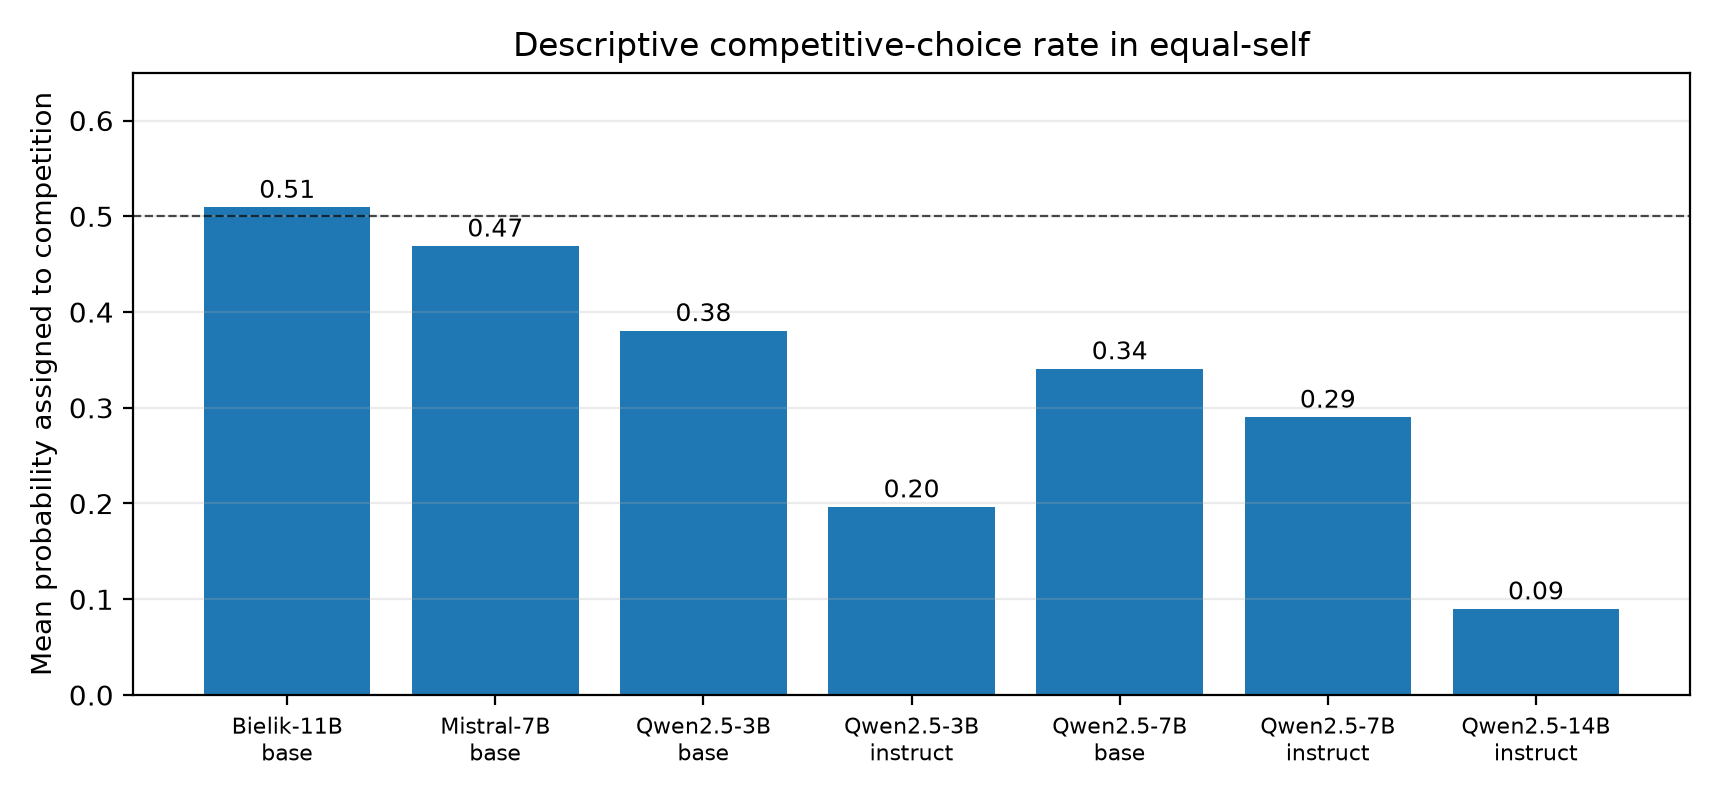
\includegraphics[width=0.82\linewidth]{figs/equal_self_rates.png}
\caption{Opisowe prawdopodobieństwo wyboru opcji rywalizacyjnej w warunku \equalself, uśrednione dla wszystkich wariantów aktora, sposobów opisu działań, języków, kontekstów sytuacyjnych, skal wypłat oraz obu kolejności prezentacji opcji, dla siedmiu wariantów, które przeszły diagnostykę. Linia przerywana oznacza poziom 0.5.}
\label{fig:equalself}
\end{figure}

\subsection{Główne efekty w warunku równych wypłat własnych}
Dodatnia wartość kontrastu oznacza wyższy logit wyboru rywalizacji w pierwszym z warunków wymienionych w danym kontraście. Oszacowania efektów oraz odpowiadające im 95\% przedziały ufności, obliczone na poziomie szablonów, przedstawiono w tabeli~\ref{tab:primaryeffects}.

\begin{table}[H]
\centering
\scriptsize
\caption{Główne kontrasty logitowe w warunku \equalself{} dla siedmiu wariantów, które przeszły diagnostykę. Wartości przedstawiono jako oszacowanie efektu wraz z 95\% przedziałem ufności (przedział $t$ po szablonach). Wartości dodatnie oznaczają wyższy logit wyboru działania rywalizacyjnego.}

\begin{tabular}{lcccc}
\toprule
Model variant & Charged $-$ plain & Tribe $-$ agent & Team $-$ agent & Scarce $-$ abundant \\
\midrule
Bielik-11B-v3 base & $-0.05\,[-0.15,0.05]$ & $0.20\,[0.08,0.31]$ & $0.08\,[-0.05,0.21]$ & $0.16\,[0.10,0.23]$ \\
Mistral-7B base & $0.38\,[0.26,0.49]$ & $-0.01\,[-0.09,0.08]$ & $0.01\,[-0.05,0.07]$ & $0.15\,[0.10,0.19]$ \\
Qwen2.5-3B base & $0.02\,[-0.09,0.13]$ & $-0.11\,[-0.24,0.03]$ & $-0.07\,[-0.15,0.01]$ & $0.21\,[0.15,0.27]$ \\
Qwen2.5-3B instruct & $0.09\,[-1.08,1.26]$ & $-0.01\,[-1.74,1.72]$ & $-1.00\,[-2.41,0.40]$ & $1.03\,[0.80,1.26]$ \\
Qwen2.5-7B base & $0.12\,[-0.00,0.24]$ & $0.21\,[0.07,0.35]$ & $0.10\,[-0.05,0.25]$ & $0.22\,[0.15,0.29]$ \\
Qwen2.5-7B instruct & $-2.26\,[-3.66,-0.85]$ & $-0.40\,[-1.97,1.16]$ & $-0.51\,[-1.84,0.82]$ & $1.93\,[1.53,2.34]$ \\
Qwen2.5-14B instruct & $-0.37\,[-1.12,0.39]$ & $1.01\,[0.12,1.89]$ & $1.07\,[0.17,1.97]$ & $0.43\,[0.07,0.79]$ \\
\bottomrule
\end{tabular}
\label{tab:primaryeffects}
\end{table}

\paragraph{H1: nacechowany i neutralny opis działań (\texttt{charged} vs. \texttt{plain}).}
Przewidywany efekt miał być ujemny: oczekiwano, że nacechowany opis działań będzie zmniejszał prawdopodobieństwo wyboru rywalizacji w porównaniu z opisem neutralnym. Zaobserwowany efekt nie jest jednak spójny między modelami. Mistral-7B Base wykazuje dodatni kontrast o wartości 0.38 ($p<0.0001$), który jest statystycznie istotnie różny od zera, ale ma kierunek przeciwny do postawionej hipotezy. W przypadku Qwen2.5-3B Base, Qwen2.5-3B-Instruct i Bielik-11B-v3 Base uzyskano oszacowania bliskie zeru, przy przedziałach ufności obejmujących zero. Wynik dla Qwen2.5-7B Base również jest bliski zeru ($p=0.0507$), a dla Qwen2.5-14B-Instruct ujemny, lecz z szerokim przedziałem ($-0.37$, $p=0.2823$). Qwen2.5-7B-Instruct wykazuje ujemne oszacowanie efektu ($-2.26$, $p=0.0061$), jednak nie spełnia ono skorygowanego progu istotności Bonferroniego wynoszącego 0.0018. W związku z tym eksperyment nie dostarcza potwierdzenia, że nacechowany opis działań w porównaniu z opisem neutralnym wywołuje efekt o przewidywanym kierunku, wspólny dla różnych modeli.

\paragraph{H2: sposób określenia aktora.}
Żaden z analizowanych kontrastów dotyczących aktora nie wykazuje stabilnego efektu we wszystkich uwzględnionych wariantach modeli i żaden nie spełnia skorygowanego progu istotności. Największe nominalne sygnały zaobserwowano dla kontrastu plemię minus agent w przypadku Bielik-11B-v3 Base ($0.20$, $p=0.0033$) i Qwen2.5-7B Base ($0.21$, $p=0.0086$); w Qwen2.5-14B-Instruct kontrasty plemię minus agent i zespół minus agent są dodatnie, lecz mają szerokie przedziały ($p=0.0295$ i $p=0.0243$). Znak kontrastów zmienia się między modelami. Biorąc pod uwagę powiązanie określeń aktora z różnymi nazwami zasobów oraz słabszą trafność kontroli numerycznych dla aktora typu agent w modelu Qwen2.5-7B-Instruct, uzyskane dane nie dostarczają solidnych dowodów na to, że same określenia aktora systematycznie wpływają na wybór rywalizacji.

\paragraph{H3: kontekst niedoboru zasobów.}
Kontrast niedobór minus obfitość zasobów (\texttt{scarce} minus \texttt{abundant}) jest dodatni we wszystkich siedmiu uwzględnionych wariantach modeli. W sześciu z nich spełnia główny, skorygowany próg istotności; wyjątkiem jest Qwen2.5-14B-Instruct ($0.43$, $p=0.0233$), gdzie przedział ufności nie obejmuje zera, ale p-wartość przekracza próg 0.0018. Oszacowane efekty mieszczą się w przedziale od 0.15 do 1.93 jednostki logitu. Odpowiadające im ilorazy szans wynoszą w przybliżeniu: 1.18 (Bielik-11B-v3-Base), 1.16 (Mistral-7B-Base), 1.23 (Qwen2.5-3B-Base), 2.80 (Qwen2.5-3B-Instruct), 1.25 (Qwen2.5-7B-Base), 6.92 (Qwen2.5-7B-Instruct) oraz 1.54 (Qwen2.5-14B-Instruct). Ilorazy te opisują zmianę szans wyboru opcji rywalizacyjnej, warunkowych względem dwóch dopuszczalnych etykiet odpowiedzi. Nie należy ich utożsamiać z bezwzględną zmianą prawdopodobieństwa.

\begin{table}[H]
\centering
\small
\caption{Bezwzględne średnie prawdopodobieństwo wyboru rywalizacji w warunku \equalself{} w kontekście niedoboru i obfitości (średnia po aktorach, opisach działań, językach, skalach i obu kolejnościach opcji) oraz różnica w punktach procentowych. Wartości opisowe, bez przedziałów ufności.}
\begin{tabular}{lccc}
\toprule
Model variant & $P(\mathrm{comp})$ scarce & $P(\mathrm{comp})$ abundant & Difference (pp) \\
\midrule
Bielik-11B-v3 base      & 0.528 & 0.490 & 3.8 \\
Mistral-7B base         & 0.486 & 0.452 & 3.4 \\
Qwen2.5-3B base         & 0.403 & 0.357 & 4.6 \\
Qwen2.5-3B instruct     & 0.231 & 0.162 & 6.9 \\
Qwen2.5-7B base         & 0.360 & 0.321 & 3.9 \\
Qwen2.5-7B instruct     & 0.354 & 0.226 & 12.9 \\
Qwen2.5-14B instruct    & 0.101 & 0.078 & 2.3 \\
\bottomrule
\end{tabular}
\label{tab:abs}
\end{table}

Tabela~\ref{tab:abs} pokazuje, że w skali prawdopodobieństwa efekt jest umiarkowany: od 2.3 do 12.9 punktu procentowego. W wariantach Base prawdopodobieństwo wyboru rywalizacji pozostaje poniżej 0.5 również w kontekście niedoboru, z wyjątkiem Bielik-11B-v3 Base, gdzie w kontekście niedoboru wynosi 0.528 (a w obfitości 0.490).

\begin{figure}[H]
\centering
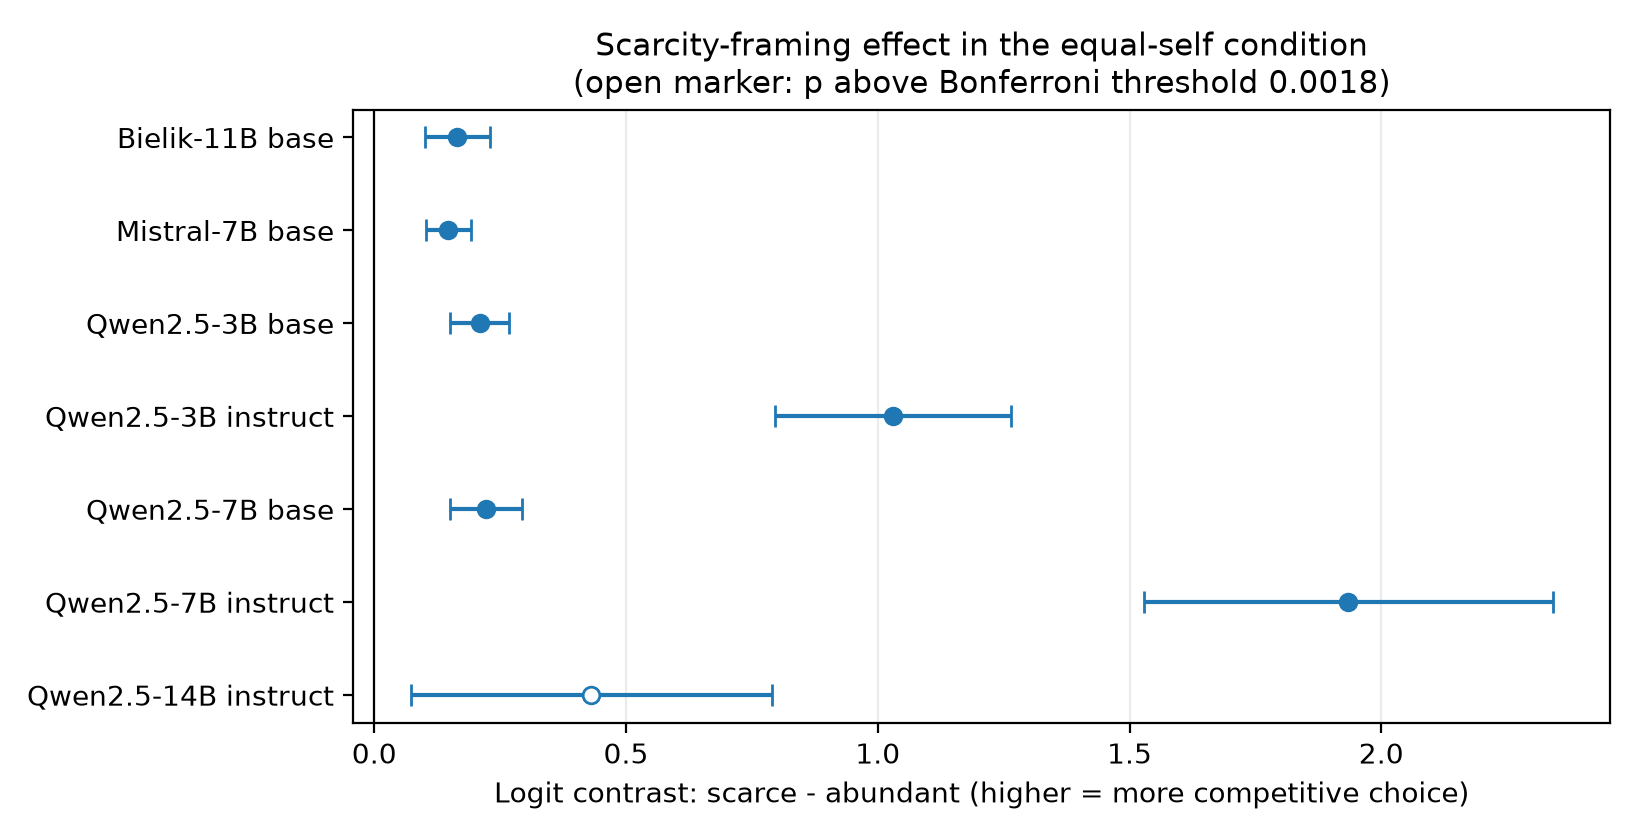
\includegraphics[width=0.82\linewidth]{figs/scarcity_effect.png}
\caption{Kontrast niedoboru zasobów względem ich obfitości w warunku \equalself{} dla siedmiu wariantów modeli, które przeszły diagnostykę poprawności pomiaru. Słupki błędów przedstawiają raportowane 95\% przedziały ufności obliczone na poziomie szablonów. Pusty znacznik oznacza p-wartość powyżej progu Bonferroniego (0.0018).}

\label{fig:scarcity}
\end{figure}

Należy zauważyć, że macierz wypłat pozostaje identyczna w warunkach niedoboru i obfitości zasobów. Zastosowana manipulacja pozwala zatem zidentyfikować wrażliwość modeli na zdanie wprowadzające kontekst niedoboru w prompcie, a nie reakcję na zmianę rzeczywistej dostępności zasobów czy struktury zachęt ekonomicznych. Zaobserwowany efekt jest stosunkowo niewielki w bazowych wariantach modeli. W Qwen2.5-3B i 7B jest wyraźnie większy w wariantach dostrojonych instrukcyjnie: różnica między efektami niedoboru dla wariantów Instruct i Base wynosi 0.82 logitu (95\% CI: [0.59; 1.06]) dla modelu 3B i 1.71 logitu (95\% CI: [1.33; 2.10]) dla modelu 7B. W Qwen2.5-14B-Instruct efekt jest natomiast mały (0.43), a wariant Base tego modelu nie przeszedł diagnostyki, więc takiej różnicy nie szacujemy. Ze względu na zastosowanie odmiennych protokołów konstruowania promptów dla modeli Base i Instruct (odpowiednio kontekst few-shot oraz format konwersacyjny bez przykładów), różnicy tej nie można przypisać przyczynowo samemu dostrajaniu instrukcyjnemu, a przy braku wzorca w kolejnych rozmiarach i rodzinach nie uogólniamy jej na dostrajanie instrukcyjne jako takie.

\subsection{Różnice między językami (analiza eksploracyjna)}\label{sec:lang}
Kontrast niedoboru jest dodatni zarówno w promptach angielskich, jak i polskich, we wszystkich siedmiu wariantach: 0.21 wobec 0.12 (Bielik-11B-v3-Base), 0.20 wobec 0.10 (Mistral-7B-Base), 0.28 wobec 0.13 (Qwen2.5-3B-Base), 1.43 wobec 0.63 (Qwen2.5-3B-Instruct), 0.22 wobec 0.22 (Qwen2.5-7B-Base), 2.52 wobec 1.34 (Qwen2.5-7B-Instruct), 0.46 wobec 0.40 (Qwen2.5-14B-Instruct). W sześciu z nich efekt jest w polskich promptach mniejszy lub równy; różnica polski minus angielski wynosi odpowiednio $-0.08$, $-0.10$, $-0.15$, $-0.80$, $0.00$, $-1.18$, $-0.06$ logitu (w kolejności jak wyżej). Nominalnie (przedziały $t$ po szablonach, bez korekcji) przedział ufności tej różnicy nie obejmuje zera w czterech wariantach (Mistral-7B Base, Qwen2.5-3B Base, Qwen2.5-3B-Instruct i Qwen2.5-7B-Instruct; najmniejsze $p=0.0037$), ale żaden z tych wyników nie spełniałby progu Bonferroniego 0.0018. Ogólny poziom logitu rywalizacji w \equalself{} różni się między językami nominalnie tylko dla Qwen2.5-7B Base ($0.53$, $p=0.0092$) i Qwen2.5-14B-Instruct ($2.76$, $p=0.0087$). Wyniki te należy traktować jako wskazówkę do dalszych badań, a nie jako potwierdzenie różnicy między językami: tłumaczenia nie były weryfikowane przez drugiego rodzimego użytkownika języka, a sześć szablonów na język daje niewielką liczbę stopni swobody.

\subsection{Przesunięcie semantyczne i wrażliwość na przewagę liczbową}

Dekompozycja wyników uzyskanych w kontrolach dominacji pozwala na dodatkową analizę wpływu sposobu opisu działań. Tabela~\ref{tab:lean} przedstawia oszacowane przesunięcie w kierunku opcji opisanej jako kooperacyjna dla każdego wariantu opisu działań, a także efekt dominacji wynikającej z wartości liczbowych wypłat, oszacowany dla warunku z neutralnymi etykietami. Dodatnia wartość parametru \texttt{lean} oznacza, że wybory modelu wykazują przesunięcie w kierunku opcji opisanej jako kooperacyjna, niezależnie od tego, która z opcji jest korzystniejsza pod względem wypłat.

\begin{table}[H]
\centering
\scriptsize
\caption{Eksploracyjna analiza przesunięcia semantycznego i wrażliwości na przewagę liczbową na podstawie prób kontrolnych z dominacją, dla siedmiu wariantów, które przeszły diagnostykę. Wartości przedstawiono jako oszacowanie efektu wraz z 95\% przedziałem ufności, w jednostkach logitu.}
\begin{tabular}{lcccc}
\toprule
Model variant & Charged lean & Label lean & Plain lean & Numbers (label) \\
\midrule
Bielik-11B-v3 base & $-0.19\,[-0.29,-0.08]$ & $0.01\,[-0.05,0.07]$ & $-0.09\,[-0.18,-0.01]$ & $0.51\,[0.34,0.68]$ \\
Mistral-7B base & $-0.03\,[-0.12,0.06]$ & $-0.02\,[-0.04,0.01]$ & $0.21\,[0.15,0.26]$ & $0.37\,[0.27,0.48]$ \\
Qwen2.5-3B base & $0.37\,[0.21,0.52]$ & $-0.01\,[-0.09,0.07]$ & $0.49\,[0.40,0.59]$ & $0.40\,[0.33,0.46]$ \\
Qwen2.5-3B instruct & $1.00\,[-0.30,2.30]$ & $0.15\,[-0.31,0.62]$ & $1.57\,[0.98,2.15]$ & $4.23\,[3.02,5.45]$ \\
Qwen2.5-7B base & $0.60\,[0.42,0.78]$ & $0.01\,[-0.05,0.07]$ & $0.64\,[0.54,0.73]$ & $0.90\,[0.74,1.05]$ \\
Qwen2.5-7B instruct & $3.89\,[2.67,5.11]$ & $-0.00\,[-0.28,0.27]$ & $1.37\,[0.78,1.97]$ & $2.90\,[2.41,3.39]$ \\
Qwen2.5-14B instruct & $7.01\,[6.19,7.82]$ & $-0.11\,[-0.41,0.20]$ & $4.11\,[3.37,4.85]$ & $5.91\,[4.57,7.24]$ \\
\bottomrule
\end{tabular}
\label{tab:lean}
\end{table}

Wariant z neutralnymi etykietami działa zgodnie z założeniami: oszacowane wartości przesunięcia semantycznego (\texttt{lean}) są bliskie zeru we wszystkich siedmiu uwzględnionych wariantach modeli (przedziały ufności obejmują zero). Wariant \texttt{plain} powoduje dodatnie przesunięcie w kierunku opcji opisanej jako kooperacyjna w sześciu z siedmiu wariantów; wyjątkiem jest Bielik-11B-v3 Base, gdzie przesunięcie jest minimalnie ujemne ($-0.09$). Wynik jest zgodny z przypuszczeniem, że same określenia „działać samodzielnie” (\texttt{independently}) i „działać wspólnie” (\texttt{jointly}) stanowią wskazówkę językową sprzyjającą wyborowi współpracy, lecz nie jest to reguła ogólna dla wszystkich modeli.

Wyniki dla wariantu \texttt{charged} są bardziej zróżnicowane. Oszacowane przesunięcie jest bliskie zeru dla Mistral-7B Base, lekko ujemne dla Bielik-11B-v3 Base ($-0.19$, czyli w stronę opcji rywalizacyjnej), dodatnie dla Qwen2.5-3B Base i Qwen2.5-7B Base, a bardzo duże dla Qwen2.5-7B-Instruct i Qwen2.5-14B-Instruct ($3.89$ i $7.01$). Oznacza to, że wariant \texttt{charged} nie działa jako prosty, niezależny od modelu czynnik związany z nacechowaniem językowym. Warto przy tym pamiętać, że w kontroli \texttt{dom\_comp} opis \texttt{charged} jest niespójny z wypłatami (por.\ ograniczenia), a wartości w Qwen2.5-14B-Instruct leżą blisko granicy skali.

\begin{figure}[H]
\centering
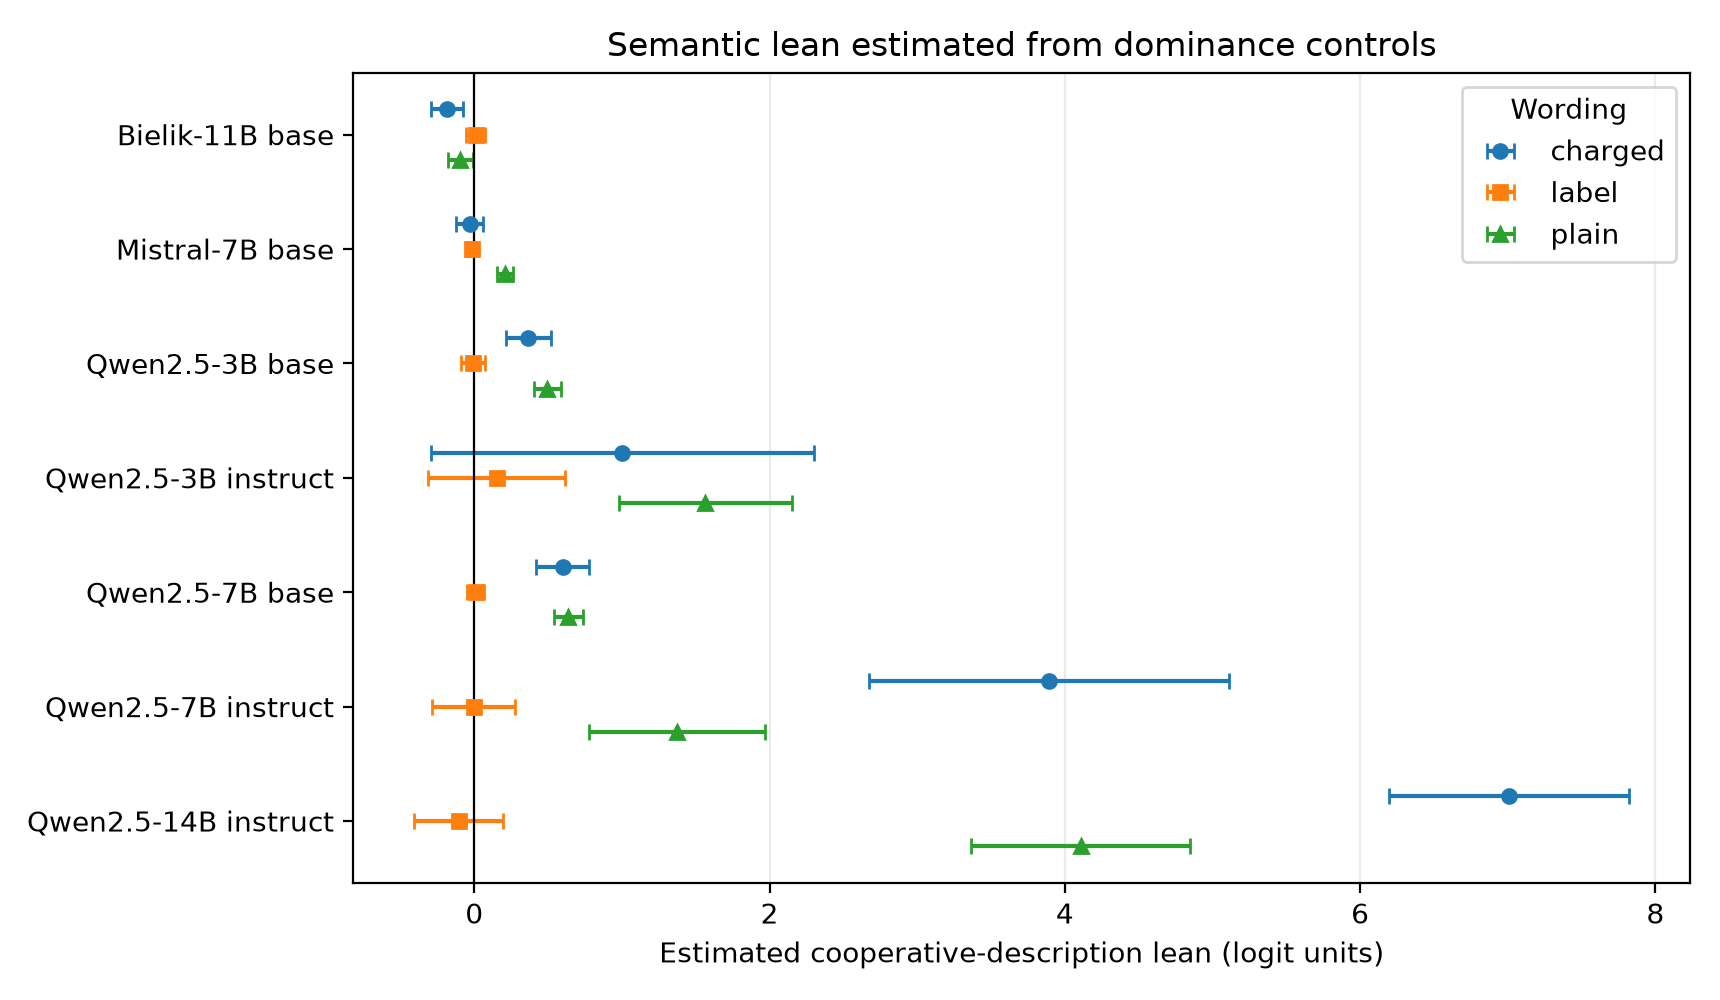
\includegraphics[width=0.92\linewidth]{figs/semantic_lean.png}
\caption{Oszacowane przesunięcie w kierunku opcji opisanej jako kooperacyjna w próbach kontrolnych z dominacją. W warunku z neutralnymi etykietami (\texttt{label}) przesunięcie jest bliskie zeru, natomiast w wariancie \texttt{plain} przyjmuje wartości dodatnie w sześciu z siedmiu uwzględnionych wariantów modeli.}
\label{fig:lean}
\end{figure}

Stosunek efektu niedoboru zasobów do efektu dominacji liczbowej, oszacowanego w warunku z neutralnymi etykietami, wynosi 0.32 dla Bielik-11B-v3-Base, 0.40 dla Mistral-7B-Base, 0.53 dla Qwen2.5-3B-Base, 0.24 dla Qwen2.5-3B-Instruct, 0.25 dla Qwen2.5-7B-Base, 0.67 dla Qwen2.5-7B-Instruct oraz 0.07 dla Qwen2.5-14B-Instruct. Są to wskaźniki opisowe, dla których nie wyznaczono przedziałów ufności. W sześciu wariantach wynoszą od 0.24 do 0.67, co wskazuje, że wpływ informacji o niedoborze zasobów nie jest pomijalny w porównaniu z wpływem jednoznacznie dominującej różnicy w wypłatach; w Qwen2.5-14B-Instruct, który bardzo silnie reaguje na liczby (\texttt{numbers} = 5.91), jest niewielki. Nie należy ich traktować jako skalibrowanych miar wyrażających wielkości na wspólnej skali psychologicznej.

Dodatkowy test spójności wewnętrznej polega na porównaniu efektów związanych ze sposobem opisu działań, przewidywanych na podstawie oszacowań przesunięcia semantycznego w próbach kontrolnych, z efektami zmierzonymi bezpośrednio w warunku \equalself{}. Przewidywane i zaobserwowane kontrasty \texttt{label} minus \texttt{plain} są dość zbliżone we wszystkich uwzględnionych wariantach modeli: $-0.10$ wobec $-0.15$ dla Bielik-11B-v3-Base, 0.23 wobec 0.27 dla Mistral-7B-Base, 0.50 wobec 0.38 dla Qwen2.5-3B-Base, 1.41 wobec 1.46 dla Qwen2.5-3B-Instruct, 0.63 wobec 0.81 dla Qwen2.5-7B-Base, 1.38 wobec 1.95 dla Qwen2.5-7B-Instruct oraz 4.21 wobec 3.83 dla Qwen2.5-14B-Instruct. W przypadku kontrastów \texttt{charged} minus \texttt{plain} zgodność jest mniej jednolita, szczególnie dla Qwen2.5-14B-Instruct ($-2.90$ wobec $-0.37$) i Qwen2.5-3B-Instruct (0.56 wobec 0.09). Test ten ma charakter opisowy i wykorzystuje ponownie dane z tego samego eksperymentu, dlatego nie stanowi niezależnej walidacji uzyskanych wyników.


\section{Dyskusja}

\subsection{Niedobór zasobów jako wskazówka kontekstowa przy niezmienionych wypłatach}

Głównym wynikiem badania jest wzrost logitu wyboru rywalizacji pod wpływem informacji o niedoborze zasobów we wszystkich siedmiu uwzględnionych wariantach modeli z trzech rodzin (Qwen2.5, Mistral, Bielik), mimo że macierz wypłat pozostaje niezmieniona; w sześciu wariantach efekt spełnia skorygowany próg istotności. Wskazuje to na powtarzalny efekt kontekstu promptu w ramach przeprowadzonego eksperymentu. Znak efektu jest dodatni także w pięciu wyłączonych wariantach (dodatek~\ref{app:sens}), co pokazuje, że wynik nie zależy od przyjętego kryterium kwalifikacji, choć wielkość efektu w tych wariantach należy interpretować ostrożnie. Wynik nie oznacza jednak, że modele doświadczają niedoboru zasobów, wykształciły ewolucyjnie uwarunkowane skłonności do rywalizacji ani że zachowywałyby się rywalizacyjnie w rzeczywistym środowisku podziału zasobów. Wyniki wskazują raczej, że warunkowe rozkłady prawdopodobieństwa kolejnego tokenu generowane przez modele są wrażliwe na wskazówkę kontekstową, która w typowym rozumieniu wiąże się z niedoborem i konfliktem.

W Qwen2.5-3B i 7B efekt jest większy w dostrojonych instrukcyjnie wariantach, lecz wzorzec ten nie powtarza się w całym zestawie: w Qwen2.5-14B-Instruct efekt jest mały (przy bardzo niskim ogólnym poziomie wyborów rywalizacyjnych), a w pozostałych rodzinach pary Base--Instruct nie przeszły diagnostyki (w surowych oszacowaniach różnice mają różne znaki). Obecny protokół eksperymentalny nie pozwala na wyizolowanie wpływu samego dostrajania instrukcyjnego. Modele bazowe otrzymują osiem przykładów few-shot ilustrujących regułę podejmowania decyzji opartą na wypłatach, podczas gdy modele dostrojone instrukcyjnie nie otrzymują analogicznych przykładów i korzystają z innego formatu odpowiedzi. W konsekwencji zaobserwowane różnice między wariantami Base i Instruct mogą wynikać z procesu trenowania modeli, przykładów dostarczonych w kontekście, formatu konwersacyjnego, sposobu zakończenia promptu lub interakcji między tymi czynnikami.

\subsection{Sposób opisu działań nie jest zmienną czysto kosmetyczną}

Wyniki kontroli dominacji wskazują, że sposób opisu dostępnych działań może wpływać na wybory modeli nawet wtedy, gdy jedna z opcji jest korzystniejsza dla obu stron. W szczególności wariant \texttt{plain} przesuwa wybory w kierunku opcji opisanej jako działanie wspólne w sześciu z siedmiu wariantów (wyjątkiem jest Bielik-11B-v3 Base, z minimalnym przesunięciem w przeciwną stronę). Zastosowanie neutralnych etykiet eliminuje to przesunięcie we wszystkich siedmiu wariantach. Ma to istotne znaczenie dla oceny zachowań modeli: eksperyment wykorzystujący wyłącznie określenia takie jak „współpracować” i „rywalizować” może w sposób niezamierzony mierzyć reakcję na skojarzenia semantyczne, zamiast wrażliwości na strukturę wypłat.

Wariant \texttt{charged} jest szczególnie trudny do interpretacji jako pojedynczy czynnik. Łączy on język wykluczenia w opisie działania rywalizacyjnego z językiem sugerującym afiliację i współdziałanie w opisie działania kooperacyjnego. Niektóre warianty modeli wykazują w tych warunkach silne przesunięcie w kierunku opcji opisanej jako kooperacyjna (w Qwen2.5-14B-Instruct niemal całkowicie przesłaniające liczby w kontroli \texttt{dom\_comp}), inne niewielkie lub żadne, a Bielik-11B-v3 Base lekko w przeciwną stronę. Wyniki przemawiają zatem za rozdzieleniem manipulacji językowych na niezależnie zmieniane elementy, takie jak nacechowanie wartościujące, sposób przedstawienia sprawczości, semantyka działania oraz jawnie wskazane konsekwencje społeczne.

\subsection{Określenia aktorów a trafność konstruktu}

Manipulacja dotycząca sposobu określenia aktora nie wykazuje stabilnego efektu w analizie głównej. Nie jest to jednak czysta manipulacja tożsamością grupową, ponieważ określenia aktorów są powiązane z różnymi nazwami zasobów. W przyszłych badaniach należałoby zachować tę samą nazwę i jednostkę zasobu, zmieniając wyłącznie określenie aktora, a także uwzględnić kilka różnych określeń w każdej kategorii pojęciowej. Pozwoliłoby to odróżnić wpływ tożsamości grupowej od wpływu słownictwa związanego z określoną dziedziną.

\subsection{Odniesienie do wcześniejszych badań}

Uzyskane wyniki uzupełniają badania wskazujące, że opisy formułowane w języku naturalnym mogą ukierunkowywać wybory modeli LLM w grach ekonomicznych \citep{phelps2025machine}, a także prace pokazujące, że zachowanie modeli w powtarzanych interakcjach strategicznych zależy od struktury gry i sposobu przedstawienia sytuacji \citep{akata2025repeated,pal2026robust}. Stanowią również uzupełnienie szerszych ocen modeli w zakresie dylematów społecznych, takich jak CoopEval, oparte na kontrolowanym zadaniu jednorazowego wyboru \citep{tewolde2026coopeval}. Kluczową różnicą jest to, że w niniejszym badaniu macierz wypłat pozostaje niezmieniona, podczas gdy manipulacji podlega informacja o niedoborze zasobów. Umożliwia to bezpośrednie zbadanie, czy zmiana kontekstu sytuacyjnego wpływa na rozkład prawdopodobieństwa wyboru w zadaniu wymuszonego wyboru.

\section{Ograniczenia badania}\label{sec:limits}

Istnieje kilka ograniczeń, które należy uwzględnić przy interpretacji wyników niniejszego eksperymentu.

\begin{enumerate}[leftmargin=1.6em,itemsep=0.25em]

    \item \textbf{Sztuczny charakter zadania i jednostronny wybór.}
    Zastosowane scenariusze mają hipotetyczny charakter i dotyczą jednorazowego wyboru między określonymi wypłatami. Nie reprezentują gier powtarzanych, jednoczesnych decyzji strategicznych ani rzeczywistych interakcji z innym agentem. Uzyskane wyniki nie pozwalają określić, jak modele zachowywałyby się w sytuacjach, w których ich działania miałyby rzeczywiste konsekwencje.

    \item \textbf{Tekstowe przedstawienie niedoboru zamiast rzeczywistego ograniczenia zasobów.}
    Warunki niedoboru i obfitości różnią się wyłącznie jednym zdaniem wprowadzającym scenariusz. Dostępność zasobów, wykonalność działań oraz struktura wypłat pozostają identyczne. Zaobserwowany efekt należy zatem opisywać jako wpływ tekstowego przedstawienia sytuacji niedoboru zasobów.

    \item \textbf{Brak neutralnego punktu odniesienia dla niedoboru.}
    Kontrast \texttt{scarce} minus \texttt{abundant} nie pozwala stwierdzić, czy niedobór zwiększa skłonność do rywalizacji, czy obfitość ją zmniejsza. Zdania obu warunków nie są też dopasowane długością ani treścią, a nie zastosowano warunku bez zdania kontekstowego ani placebo.

    \item \textbf{Różnice w sposobie konstruowania promptów dla wariantów Base i Instruct.}
    Modele bazowe otrzymują przykłady few-shot, natomiast modele dostrojone instrukcyjnie korzystają z szablonów konwersacyjnych i nie otrzymują odpowiadających im przykładów demonstracyjnych. W konsekwencji różnic między tymi wariantami nie można interpretować jako przyczynowych efektów samego dostrajania instrukcyjnego. Przykłady few-shot uczą ponadto głównie maksymalizacji wypłaty własnej (por.\ rozdz.~3.4).

    \item \textbf{Selekcja modeli przez kryterium poprawności i skromna liczba rodzin.}
    Do analizy głównej zakwalifikowano 7 z 12 wariantów, przy czym żaden wariant Instruct spoza rodziny Qwen2.5 nie przeszedł kontroli. W analizie głównej nie ma więc kompletnych par Base--Instruct dla Mistrala, Bielika, Gemmy ani Qwen2.5-14B. Kryterium trafności opiera się na 48 parach na komórkę, więc różnice rzędu 1--3 par są szumem. Wyniki dla wariantów wyłączonych zestawiono w dodatku, aby czytelnik mógł ocenić wpływ selekcji.

    \item \textbf{Wpływ kwantyzacji i precyzji na porównywalność modeli.}
    Modele Qwen2.5-3B i Gemma-4-12B są oceniane z precyzją FP16, natomiast Qwen2.5-7B, Qwen2.5-14B, Mistral-7B i Bielik-11B wykorzystują kwantyzację 4-bitową. Porównania modeli o różnej liczbie parametrów łączą zatem wpływ skali modelu z różnicami w precyzji numerycznej.

    \item \textbf{Ograniczona liczba szablonów.}
    Raportowane przedziały ufności na poziomie szablonów opierają się na zaledwie sześciu parafrazach dla każdego języka. Przedziały te nie uwzględniają niepewności wynikającej z różnic między checkpointami modeli, promptami spoza zastosowanej rodziny szablonów ani wielokrotnym stochastycznym generowaniem odpowiedzi.

    \item \textbf{Zmiany kryteriów poprawności pomiaru, historia formułowania hipotez i kolejność dodawania modeli.}
    Hipotezy H1 i H3 zostały sformułowane na podstawie wcześniejszych obserwacji eksperymentalnych, a kryterium kwalifikacji modeli zastosowane od wersji v3.2 zmodyfikowano po zapoznaniu się z wynikami wcześniejszej analizy v3 (kryterium nie było już zmieniane po dodaniu modeli Bielik i Gemma w v3.4). Modele dodawano w kolejnych przebiegach: najpierw Qwen2.5-3B i 7B, potem Mistral-7B, następnie Qwen2.5-14B, a w wersji v3.4 Bielik-11B-v3 i Gemma-4-12B. Prefill „Answer:”/„Odpowiedź:” dla Mistral-Instruct wprowadzono po stwierdzeniu, że model ten nie zwraca litery odpowiedzi jako pierwszego tokenu; ostatecznie i tak został wykluczony. Uzyskane wyniki należy zatem traktować jako rezultat powtórzenia wcześniejszych obserwacji na nowych parafrazach, a nie jako w pełni konfirmacyjne badanie oparte na uprzednio zarejestrowanym planie eksperymentalnym i analitycznym.

    \item \textbf{Złożony charakter manipulacji dotyczących aktora i sposobu opisu działań.}
    Określenia aktorów są powiązane z różnymi nazwami zasobów, a oznaczenia „Agent A/B” pokrywają się z literami odpowiedzi A/B, natomiast wariant \texttt{charged} łączy kilka wymiarów semantycznych. Zastosowany projekt nie pozwala zatem na ich jednoznaczne wyodrębnienie i niezależną ocenę.

    \item \textbf{Niespójność kontroli \texttt{dom\_comp} dla opisu \texttt{charged}.}
    W warunku \texttt{dom\_comp} druga strona otrzymuje maksymalną wypłatę, podczas gdy opis działania rywalizacyjnego mówi o wypchnięciu drugiej strony. Oszacowania \texttt{lean} dla wariantu \texttt{charged} mieszają więc efekt semantyczny z niespójnością opisu i wypłat.

    \item \textbf{Efekty podłogi i obcięcie prawdopodobieństw.}
    W Qwen2.5-14B-Instruct średnie prawdopodobieństwo wyboru rywalizacji w \equalself{} wynosi zaledwie około 0.09, a w niektórych komórkach (np.\ opis \texttt{charged}) jest bliskie zeru. Obcięcie prawdopodobieństw do $10^{-4}$ ogranicza logit do około $\pm9.21$ i może tłumić kontrasty w takich komórkach.

    \item \textbf{Warunkowy charakter pomiaru odpowiedzi A/B.}
    Prawdopodobieństwa są normalizowane względem dopuszczalnych wariantów tokenów A i B. Wartość diagnostyczna \texttt{mass} jest wysoka dla modeli uwzględnionych w analizie, jednak zastosowana procedura nie ocenia swobodnie generowanych wyjaśnień ani nie pozwala stwierdzić, czy model dokonałby takiego samego wyboru podczas generowania tekstu bez ograniczenia formatu odpowiedzi. Dla modeli Instruct z prefillem (Mistral, Gemma) format końcówki promptu mógł ponadto odbiegać od typowego użycia.

    \item \textbf{Szum numeryczny w kwantyzacji 4-bitowej.}
    Zgodność oceny wsadowej i pojedynczej sprawdzono na losowej próbce 24 promptów (po jednej na wariant) dla pięciu wariantów z analizy głównej. Maksymalna bezwzględna różnica logitu $A-B$ wynosi 0.016 dla Qwen2.5-3B Base (FP16) oraz 0.188, 0.187, 0.50 i 0.75 dla modeli 4-bitowych: Qwen2.5-7B Base, Mistral-7B Base, Bielik-11B-v3 Base i Qwen2.5-14B-Instruct; dla wyłączonego Mistral-7B-Instruct 0.60 (0.76 w wcześniejszym uruchomieniu). Masy A/B w obu trybach zgadzają się z dokładnością do 0.002. Nie raportowano różnic średnich, a próbka jest mała. W Qwen2.5-14B-Instruct i Bielik-11B-v3 Base maksymalna różnica jest tego samego rzędu lub większa niż oszacowany efekt niedoboru (odpowiednio 0.43 i 0.16), więc wpływu szumu zależnego od składu paczki nie można wykluczyć; w pozostałych wariantach jest on wyraźnie mniejszy od efektu lub porównywalny. Dla wyłączonego Gemma-4-12B-Instruct (FP16) kontrola wykazała poważną rozbieżność: masa A/B wynosi 0.667 w paczkach i 0.833 przy ocenie pojedynczej, a maksymalna różnica logitu 12.7; także w ocenie pojedynczej część promptów ma masę znacznie poniżej 1. Wskazuje to na błąd oceny wsadowej lub formatu promptu dla tego modelu i może wyjaśniać jego niską trafność w kontrolach. Gemma-4-12B-Base nie została sprawdzona, więc nie wiemy, czy problem dotyczy także jej; nie sprawdzono również Bielik-Instruct i Qwen2.5-14B-Base.

    \item \textbf{Walidacja językowa i użycie AI.}
    Polskie prompty nie zostały zweryfikowane przez niezależnego rodzimego użytkownika języka. Eksperyment i tekst przygotowano z pomocą asystenta AI (Claude); odpowiedzialność za treść ponosi autor.

    \item \textbf{Niekompletna dokumentacja umożliwiająca reprodukcję eksperymentu.}
    Dostarczone materiały obejmują kod generowania promptów i przeprowadzania pomiarów oraz zestawienia zbiorcze wyników, nie zawierają jednak dokładnych identyfikatorów rewizji modeli wykorzystanych podczas pierwotnego przebiegu ani kompletnego pliku blokującego wersje środowiska programistycznego (\textit{environment lockfile}). Modele Bielik i Gemma mogą wymagać zgody na dostęp w serwisie Hugging Face. Niezależna ponowna analiza danych oraz dokładne odtworzenie eksperymentu wymagają udostępnienia tych materiałów.

\end{enumerate}

\section{Wnioski}

W przeprowadzonym, kontrolowanym zadaniu decyzyjnym obejmującym dwie strony i określone wypłaty informacja o niedoborze zasobów zwiększa logit wyboru rywalizacji w warunku równych wypłat własnych (\equalself{}) we wszystkich siedmiu wariantach modeli, które spełniły przyjęte kryteria diagnostyczne poprawności pomiaru (w sześciu z nich po korekcji Bonferroniego), a znak efektu jest dodatni także w wariantach wyłączonych. Efekt jest najsilniejszy w dostrojonych instrukcyjnie wariantach Qwen2.5-3B i 7B, jednak zastosowany protokół eksperymentalny nie pozwala przypisać tej różnicy wyłącznie dostrajaniu instrukcyjnemu, a w Qwen2.5-14B-Instruct efekt jest mały. Efekty związane z określeniem aktora nie wykazują powtarzalnego wzorca, a hipoteza dotycząca różnicy między nacechowanym i neutralnym opisem działań (\texttt{charged} vs. \texttt{plain}) nie znajduje spójnego potwierdzenia w badanych modelach. Kontrole dominacji wskazują ponadto, że samo użycie określeń takich jak „działać samodzielnie” i „działać wspólnie” może przesuwać wybory w kierunku opcji opisanej jako kooperacyjna, nawet wtedy, gdy przewagę pod względem liczbowym ma druga opcja (sześć z siedmiu wariantów).

Szersze znaczenie uzyskanych wyników ma przede wszystkim charakter metodologiczny: ocena zachowań decyzyjnych modeli językowych w sytuacjach społecznych wymaga rozdzielenia rozumienia struktury wypłat od wpływu kontekstu sytuacyjnego i semantycznego opisu dostępnych działań. Pozorna skłonność modelu do współpracy lub rywalizacji może ulegać znaczącym zmianom, gdy konsekwencje liczbowe pozostają niezmienione, a zmienia się jedynie otaczający je kontekst językowy. Wyniki te dotyczą wąskiej grupy modeli i jednego zadania; wskazują one na wpływ treści promptu na rozkłady prawdopodobieństwa wyboru modelu, a nie na istnienie jego trwałych preferencji lub autonomicznych motywacji.


\section*{Informacja o odtwarzalności eksperymentu}

% TODO przed publikacją: zdeponować materiały i wpisać adres repozytorium.
Implementacja generatora promptów oraz procedur pomiaru i analizy (notebook v3.4) odpowiada przebiegowi, którego wyniki przedstawiono w pracy. Surowy plik \texttt{results\_raw\_v3.csv} (41\,472 wiersze, dwanaście wariantów modeli), wyeksportowane tabele efektów i \texttt{lean}, dokładne identyfikatory rewizji modeli oraz środowisko z przypiętymi wersjami oprogramowania nie są jeszcze udostępnione publicznie. Analiza z notebooka odtwarza wartości z tabel na podstawie surowego pliku wyników. Niniejszy manuskrypt nie deklaruje, że brakujące artefakty z pierwotnego przebiegu zostały niezależnie odtworzone.


\appendix
\section{Analiza wrażliwości: wszystkie dwanaście wariantów}\label{app:sens}
Tabela~\ref{tab:sens} zestawia kontrast niedoboru zasobów dla wszystkich wariantów, także tych, które nie przeszły diagnostyki. Wartości dla wariantów oznaczonych ``No'' nie podlegają interpretacji merytorycznej, a podajemy je, aby pokazać, że wynik nie wynika z selekcji modeli. Znak efektu jest dodatni w dwunastu z dwunastu wariantów, a przedział ufności nie obejmuje zera w jedenastu (wyjątek: Gemma-4-12B Instruct, którego pomiar jest niewiarygodny). Wielkość efektu bywa duża (np.\ Gemma-4-12B Base), co przy niskiej trafności kontroli numerycznych nie powinno być czytane jako wynik substancjalny. Różnice Instruct$-$Base w surowych oszacowaniach mają różne znaki (np.\ Bielik-11B-v3 $+1.83$, Mistral-7B $+0.70$, Qwen2.5-14B $-0.09$, Gemma-4-12B $-2.61$ logitu), co dodatkowo przemawia przeciw uogólnianiu wzorca z Qwen2.5-3B i 7B.

\begin{table}[H]
\centering
\scriptsize
\caption{Kontrast \texttt{scarce} $-$ \texttt{abundant} w warunku \equalself{} dla wszystkich dwunastu wariantów (logity, 95\% przedział $t$ po szablonach), p-wartość niekorygowana oraz średnie $P(\mathrm{comp})$ w kontekście niedoboru i obfitości.}
\begin{tabular}{lccccc}
\toprule
Model variant & Scarce $-$ abundant & $p$ & $P$ scarce & $P$ abundant & Retained \\
\midrule
Bielik-11B-v3 base      & $0.16\,[0.10,0.23]$ & 0.0003 & 0.528 & 0.490 & Yes \\
Bielik-11B-v3 instruct  & $1.99\,[1.51,2.48]$ & <0.0001 & 0.531 & 0.366 & No \\
Gemma-4-12B base        & $2.71\,[1.98,3.44]$ & <0.0001 & 0.618 & 0.358 & No \\
Gemma-4-12B instruct    & $0.10\,[-0.44,0.64]$ & 0.6743 & 0.584 & 0.569 & No \\
Mistral-7B base         & $0.15\,[0.10,0.19]$ & <0.0001 & 0.486 & 0.452 & Yes \\
Mistral-7B instruct     & $0.85\,[0.21,1.48]$ & 0.0185 & 0.508 & 0.462 & No \\
Qwen2.5-3B base         & $0.21\,[0.15,0.27]$ & <0.0001 & 0.403 & 0.357 & Yes \\
Qwen2.5-3B instruct     & $1.03\,[0.80,1.26]$ & <0.0001 & 0.231 & 0.162 & Yes \\
Qwen2.5-7B base         & $0.22\,[0.15,0.29]$ & <0.0001 & 0.360 & 0.321 & Yes \\
Qwen2.5-7B instruct     & $1.93\,[1.53,2.34]$ & <0.0001 & 0.354 & 0.226 & Yes \\
Qwen2.5-14B base        & $0.52\,[0.41,0.63]$ & <0.0001 & 0.428 & 0.332 & No \\
Qwen2.5-14B instruct    & $0.43\,[0.07,0.79]$ & 0.0233 & 0.101 & 0.078 & Yes \\
\bottomrule
\end{tabular}
\label{tab:sens}
\end{table}

\begin{thebibliography}{9}

\bibitem{phelps2025machine}
S. Phelps and Y. I. Russell.
\newblock The machine psychology of cooperation: can {\sc GPT} models operationalize prompts for altruism, cooperation, competitiveness, and selfishness in economic games?
\newblock \emph{Journal of Physics: Complexity}, 6(1):015018, 2025.
\newblock doi:10.1088/2632-072X/ada711.

\bibitem{akata2025repeated}
E. Akata, L. Schulz, J. Coda-Forno, S. J. Oh, M. Bethge, and E. Schulz.
\newblock Playing repeated games with large language models.
\newblock \emph{Nature Human Behaviour}, 9(7):1380--1390, 2025.
\newblock doi:10.1038/s41562-025-02172-y.

\bibitem{tewolde2026coopeval}
E. Tewolde, X. Zhang, D. Guzman Piedrahita, V. Conitzer, and Z. Jin.
\newblock {\sc CoopEval}: Benchmarking cooperation-sustaining mechanisms and {\sc LLM} agents in social dilemmas.
\newblock In \emph{Proceedings of the 43rd International Conference on Machine Learning}, volume 306 of \emph{Proceedings of Machine Learning Research}, pages 120222--120287, 2026.

\bibitem{pal2026robust}
S. Pal, A. Mallela, L. Pracher, C. Wei, F. Fu, S. Schnell, and M. A. Nowak.
\newblock Large language models instantiate evolutionarily robust strategies of cooperation.
\newblock \emph{PNAS Nexus}, 5(6):pgag210, 2026.
\newblock doi:10.1093/pnasnexus/pgag210.

\end{thebibliography}

\end{document}
